% This is text associated with the open textbook "Open Electromagnetics"
% See immediately below for author, date
% This work is licensed under the Creative Commons Attribution-ShareAlike 4.0 International License. (CC BY-SA 4.0) 
% To view a copy of the license, visit http://creativecommons.org/licenses/by-sa/4.0/

%ORB TITLE Attenuation in Coaxial Cable
%ORB AUTHOR 0        # S.W. Ellingson, Virginia Tech (ellingson@vt.edu)
%ORB DATE 20191122   # yyyymmdd
%ORB ABSTRACT  

\label{m0189_Attenuation_Coaxial_Cable} % <-- Must match name of this file and module directory name.  Don't mess with this!
\index{transmission line!coaxial|(}
\index{attenuation|(}

In this section, we consider the issue of attenuation in coaxial transmission line.
Recall that attenuation can be interpreted in the context of the ``lumped element'' equivalent circuit transmission line model as the contributions of the resistance per unit length $R'$ and conductance per unit length $G'$.
In this model, $R'$ represents the physical resistance in the inner and outer conductors, whereas $G'$ represents loss due to current flowing directly between the conductors through the spacer material. 

The parameters used to describe the relevant features of coaxial cable are shown in Figure~\ref{m0189_f1}. 
In this figure, $a$ and $b$ are the radii of the inner and outer conductors, respectively.
$\sigma_{ic}$ and $\sigma_{oc}$ are the conductivities (SI base units of S/m) of the inner and outer conductors, respectively.
Conductors are assumed to be non-magnetic; i.e., having permeability $\mu$ equal to the free space value $\mu_0$.
The spacer material is assumed to be a lossy dielectric having relative permittivity $\epsilon_r$ and conductivity $\sigma_s$.
%
\begin{figure}[b!] % <--- "[b!]" for first figure in section *only*; delete for 2nd and subsequent figures
\begin{center}
\pdftooltip{{  % note double braces
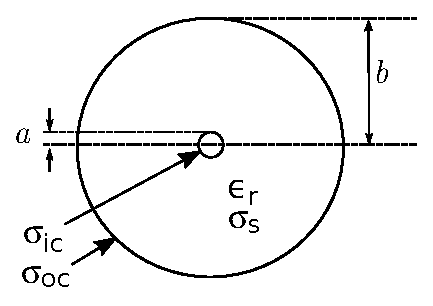
\includegraphics[width=2in]{modules/m0189_f1.eps} 
% https://commons.wikimedia.org/wiki/File:M0003_fBarMagnet.svg
}}{Diagram of two concentric circles, where the inner circle is labeled, small sigma subscript quantity i c. The outer circle is labeled small sigma subscript quantity o c. The radius of the inner circle is small a and the radius of the outer circle is small b. Dielectric material small epsilon subscript r and small sigma subscript s.}
\end{center}
%\centerline{\scriptsize 
%\copyright~\hyperref[m0003_fBarMagnet_Credit]{Y.\ Qin} 
%\href{https://creativecommons.org/licenses/by/3.0/}{CC BY 3.0} 
%} % \centerline 
\caption{
\label{m0189_f1}
Parameters defining the design of a coaxial cable.
}
\end{figure}

%%%%%%%%%%%%%%%%%%%%%%%%%%%%%%%%%%%%%%%%%%%%%%%%%%%%%
{\bf Resistance per unit length.}   
The resistance per unit length is the sum of the resistances of the inner and outer conductor per unit length.  
The resistance per unit length of the inner conductor is determined by $\sigma_{ic}$ and the effective cross-sectional area through which the current flows. 
The latter is equal to the circumference $2\pi a$ times the skin depth 
\index{skin depth}
$\delta_{ic}$ of the inner conductor, so:
%
\begin{equation}
R_{ic}' \approx \frac{1}{\left(2\pi a \cdot \delta_{ic} \right) \sigma_{ic} } ~~~ \mbox{for} ~ \delta_{ic} \ll a 
\end{equation}
% 
This expression is only valid for $\delta_{ic} \ll a$ because otherwise the cross-sectional area through which the current flows is not well-modeled as a thin ring near the surface of the conductor.  
Similarly, we find the resistance per unit length of the outer conductor is
%
\begin{equation} 
R_{oc}' \approx \frac{1}{\left(2\pi b \cdot \delta_{oc} \right) \sigma_{oc} } ~~~ \mbox{for} ~ \delta_{oc} \ll t 
\end{equation}
%
where $\delta_{oc}$ is the skin depth of the outer conductor and $t$ is the thickness of the outer conductor.
Therefore, the total resistance per unit length is
%
\begin{flalign} 
R' &= R_{ic}' + R_{oc}' \nonumber \\
   & \approx \frac{1}{\left(2\pi a \cdot \delta_{ic} \right) \sigma_{ic} } 
           + \frac{1}{\left(2\pi b \cdot \delta_{oc} \right) \sigma_{oc} } \label{m0189_eRp1} 
\end{flalign}
%
Recall that skin depth depends on conductivity.
Specifically:
%
\begin{flalign}
\delta_{ic} &= \sqrt{2/\omega\mu\sigma_{ic}} \\
\delta_{oc} &= \sqrt{2/\omega\mu\sigma_{oc}} 
\end{flalign}
%
Expanding Equation~\ref{m0189_eRp1} to show explicitly the dependence on conductivity, we find:
%
\begin{equation}
R' \approx \frac{1}{2\pi \sqrt{2/\omega\mu_0} }
\left[
\frac{1}{a \sqrt{\sigma_{ic}} } + \frac{1}{b \sqrt{\sigma_{oc}} }
\right]
\end{equation}
%
At this point it is convenient to identify two particular cases for the design of the cable.  
In the first case, ``Case~I,'' we assume $\sigma_{oc} \gg \sigma_{ic}$.  
Since $b > a$, we have in this case
%
\begin{flalign}
R' &\approx  \frac{1}{2\pi \sqrt{2/\omega\mu_0} } \left[ \frac{1}{a \sqrt{\sigma_{ic}} }  \right] \nonumber \\
   &= \frac{1}{2\pi \delta_{ic} \sigma_{ic} }~\frac{1}{a} ~~~\mbox{(Case~I)}
\end{flalign}
%
In the second case, ``Case~II,'' we assume $\sigma_{oc} = \sigma_{ic}$.  
In this case, we have
%
\begin{flalign}
R' &\approx \frac{1}{2\pi \sqrt{2/\omega\mu_0} } \left[ \frac{1}{a \sqrt{\sigma_{ic}} } + \frac{1}{b \sqrt{\sigma_{ic}} }  \right] \nonumber \\
   &= \frac{1}{2\pi \delta_{ic} \sigma_{ic} }~\left[ \frac{1}{a} + \frac{1}{b} \right]  ~~~\mbox{(Case~II)}
\end{flalign}
%
A simpler way to deal with these two cases is to represent them both using the single expression
%
\begin{equation}
R' \approx \frac{1}{2\pi \delta_{ic} \sigma_{ic} }~\left[ \frac{1}{a} + \frac{C}{b} \right]
\end{equation}
%
where $C=0$ in Case~I and $C=1$ in Case~II. 

{\bf Conductance per unit length.}
The conductance per unit length of coaxial cable is simply that of the associated coaxial structure at DC; i.e.,
%
\begin{equation}
G' = \frac{2\pi\sigma_s}{\ln\left(b/a\right)}
\end{equation}
%
Unlike resistance, the conductance is independent of frequency, at least to the extent that $\sigma_s$ is independent of frequency.

%========================================================
{\bf Attenuation.}
The attenuation of voltage and current waves as they propagate along the cable is represented by the factor $e^{-\alpha z}$, where $z$ is distance traversed along the cable. 
It is possible to find an expression for $\alpha$ in terms of the material and geometry parameters using:
%
\begin{equation}
\gamma \triangleq \sqrt{ \left( R' + j\omega L' \right) \left( G' + j\omega C' \right)} = \alpha + j\beta 
\label{m0189_fGamma}
\end{equation}
%
where $L'$ and $C'$ are the inductance per unit length and capacitance per unit length, respectively.
These are given by
%
\begin{equation}
L' = \frac{\mu}{2\pi}\ln{\left(b/a\right)}
\end{equation}
%
and
%
\begin{equation}
C' = \frac{2\pi\epsilon_0\epsilon_r}{\ln{\left(b/a\right)}}
\end{equation}
%
In principle we could solve Equation~\ref{m0189_fGamma} for $\alpha$.  
However, this course of action is quite tedious, and a simpler approximate approach facilitates some additional insights. 
In this approach, we define parameters $\alpha_R$ associated with $R'$ and $\alpha_G$ associated with $G'$ such that
%
\begin{equation}
e^{-\alpha_R z} e^{-\alpha_G z} = e^{-\left(\alpha_R+\alpha_G\right) z} = e^{-\alpha z} 
\end{equation}
%
which indicates 
%
\begin{equation}
\alpha = \alpha_R + \alpha_G
\end{equation}
%
Next we postulate 
%
\begin{equation}
\alpha_R \approx K_R \frac{R'}{Z_0} 
\label{m0189_eAlphaR}
\end{equation}
%
where $Z_0$ is the characteristic impedance 
%
\begin{equation}
Z_0 \approx \frac{\eta_0}{2\pi}\frac{1}{\sqrt{\epsilon_r}}\ln{\frac{b}{a}}~~~\mbox{(low loss)}
\label{m0189_eZ0cc}
\end{equation}
%
and where $K_R$ is a unitless constant to be determined.
The justification for Equation~\ref{m0189_eAlphaR} is as follows: 
First, $\alpha_R$ must increase monotonically with increasing $R'$.
Second, $R'$ must be divided by an impedance in order to obtain the correct units of 1/m.
Using similar reasoning, we postulate
%
\begin{equation}
\alpha_G \approx K_G G' Z_0
\label{m0189_eAlphaG}
\end{equation}
%
where $K_G$ is a unitless constant to be determined.
The following example demonstrates the validity of Equations~\ref{m0189_eAlphaR} and \ref{m0189_eAlphaG}, and will reveal the values of $K_R$ and $K_G$.

%%%%%%%%%%%%%%%%%%%%%%%%%%%%%%%%%%%%%%%%%%%%%%%
%ORB EXAMPLE
~\\ \begin{example} 
\label{m0189_exRG59}
\begin{mdframed}[backgroundcolor=brown!20,linecolor=brown!20]\raggedright
Attenuation constant for RG-59.
\index{RG-59}
\\~\\
RG-59 is a popular form of coaxial cable having the parameters
$a \cong 0.292~$mm,
$b \cong 1.855$~mm,
$\sigma_{ic} \cong 2.28 \times 10^7$~S/m,
$\sigma_s \cong 5.9 \times 10^{-5}$~S/m, and
$\epsilon_r \cong 2.25$.
The conductivity $\sigma_{oc}$ of the outer conductor is difficult to quantify because it consists of a braid of thin metal strands.
However, $\sigma_{oc}\gg\sigma_{ic}$, so we may assume Case~I; i.e., $\sigma_{oc}\gg\sigma_{ic}$, and subsequently $C=0$.  
Figure~\ref{m0189_fAlpha} shows the components $\alpha_G$ and $\alpha_R$ computed for the particular choice $K_R=K_G=1/2$.
The figure also shows $\alpha_G + \alpha_R$, along with $\alpha$ computed using Equation~\ref{m0189_fGamma}.
We find that the agreement between these values is very good, which is compelling evidence that the ansatz is valid and $K_R=K_G=1/2$. 
\end{mdframed}
% note figures will need to go between "\end{mdframed}" and "\end{example}"
%
\begin{figure} % <--- "[b!]" for first figure in section *only*; delete for 2nd and subsequent figures
\begin{center}
\pdftooltip{{  % note double braces
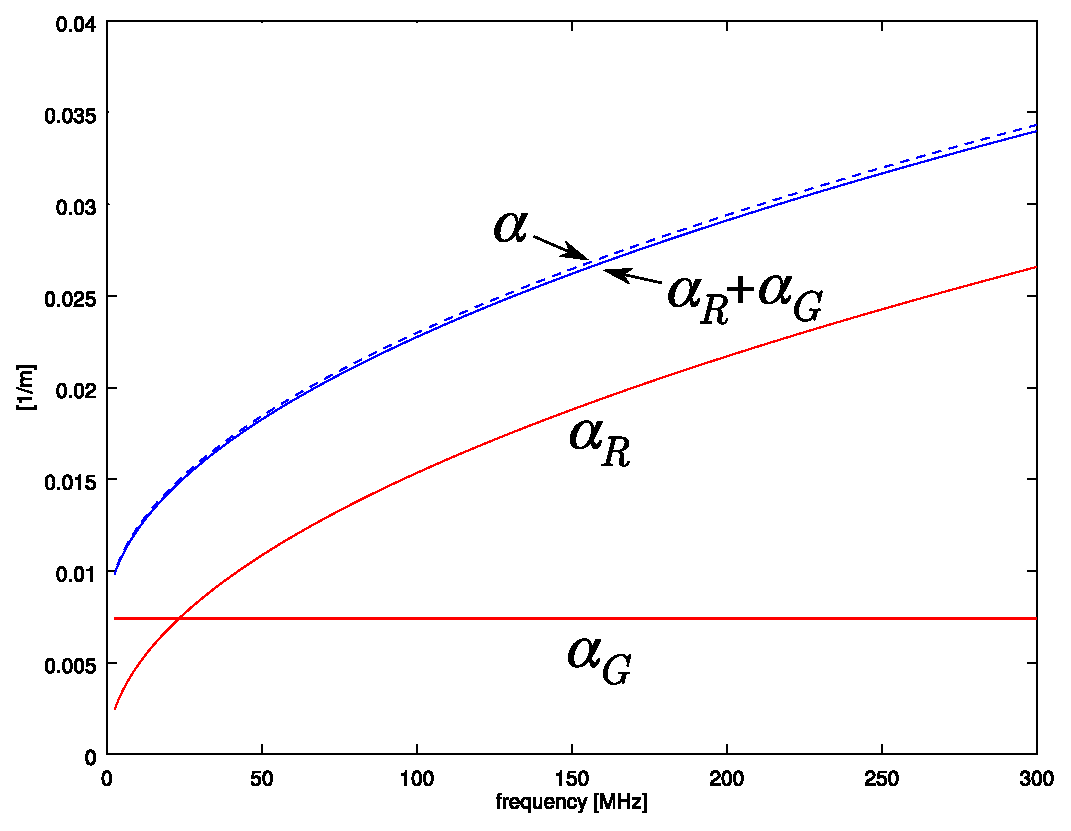
\includegraphics[width=3.2in]{modules/m0189_fAlpha.eps} 
% https://commons.wikimedia.org/wiki ...
}}{An x-y plot with x-axis of frequency in megahertz has a range of 0 to 300 measured in increments of 50. The y-axis in 1 over small m has a range of 0 to 0.04 measured in increments of 0.005. There are four lines plotted. Line alpha subscript g is a flat horizontal line at y = 0.0075. Line alpha subscript r has a y-intercept near zero; it is a convex curve with a positively increasing slope that becomes progressively more linear. The line labeled alpha subscript capital r plus alpha subscript capital g runs parallel to alpha. They have a y-intercept near 0.01 and form a convex curve with a positively increasing slope.}
\end{center}
%\centerline{\scriptsize 
%\copyright~\hyperref[m0003_fBarMagnet_Credit]{Y.\ Qin} 
%\href{https://creativecommons.org/licenses/by/3.0/}{CC BY 3.0} 
%} % \centerline 
\caption{
\label{m0189_fAlpha}
Comparison of $\alpha=\mbox{Re}\left\{\gamma\right\}$ to $\alpha_R$, $\alpha_G$, and $\alpha_R+\alpha_G$ for $K_R=K_G=1/2$.  The result for $\alpha$ has been multiplied by 1.01; otherwise the curves would be too close to tell apart.
}
\end{figure}
%
\end{example}
%%%%%%%%%%%%%%%%%%%%%%%%%%%%%%%%%%%%%%%%%%%%%%%

Note that there is nothing to indicate that the results demonstrated in the example are not generally true.
Thus, we come to the following conclusion:

%%%%%%%%%%%%%%%%%%%%%%%%%%%%%%%%%%%%%%%%%%%%%%%
%ORB HIGHLIGHT
\begin{mdframed}[backgroundcolor=yellow!20,nobreak=true] 
The attenuation constant $\alpha\approx\alpha_G+\alpha_R$ where 
$\alpha_G\triangleq R'/2Z_0$ and
$\alpha_R\triangleq G'Z_0/2$.
\end{mdframed}
%%%%%%%%%%%%%%%%%%%%%%%%%%%%%%%%%%%%%%%%%%%%%%%

%========================================================
{\bf Minimizing attenuation.}
Let us now consider if there are design choices which minimize the attenuation of coaxial cable.  
Since $\alpha=\alpha_R+\alpha_G$, we may consider $\alpha_R$ and $\alpha_G$ independently.  
Let us first consider $\alpha_G$:
%
\begin{flalign}
\alpha_G &\triangleq \frac{1}{2}G'Z_0 \nonumber \\
         &\approx \frac{1}{2} \cdot \frac{2\pi\sigma_s}{\ln\left(b/a\right)} \cdot \frac{1}{2\pi} \frac{\eta_0}{\sqrt{\epsilon_r}} \ln\left(b/a\right) \nonumber \\
         &= \frac{\eta_0}{2}~\frac{\sigma_s}{\sqrt{\epsilon_r}}
\end{flalign}
%
It is clear from this result that $\alpha_G$ is minimized by minimizing $\sigma_s/\sqrt{\epsilon_r}$.
Interestingly the physical dimensions $a$ and $b$ have no discernible effect on $\alpha_G$.\\

\noindent
Now we consider $\alpha_R$:
%
\begin{flalign}
\alpha_R  &\triangleq \frac{R'}{2Z_0} \nonumber \\
          & = \frac{1}{2} \frac{ \left(1/ 2\pi \delta_{ic} \sigma_{ic}\right)\left[ 1/a + C/b \right] }{ \left(1/2\pi\right) \left( \eta_0/\sqrt{\epsilon_r} \right) \ln\left(b/a\right) } \nonumber \\
          &= \frac{\sqrt{\epsilon_r}}{2\eta_0\delta_{ic} \sigma_{ic}} \cdot \frac{ \left[ 1/a + C/b \right] }{  \ln\left(b/a\right) }
\end{flalign}
%
Now making the substitution $\delta_{ic} = \sqrt{2/\omega\mu_0\sigma_{ic}}$ in order to make the dependences on the constitutive parameters explicit, we find:
%
\begin{equation}
\alpha_R = \frac{1}{2\sqrt{2}\cdot\eta_0} \sqrt{\frac{\omega\mu_0 \epsilon_r}{\sigma_{ic}}} \cdot \frac{ \left[ 1/a + C/b \right] }{  \ln\left(b/a\right) }
\end{equation}
%
Here we see that $\alpha_R$ is minimized by minimizing $\epsilon_r/\sigma_{ic}$.
It's not surprising to see that we should maximize $\sigma_{ic}$.  
However, it's a little surprising that we should minimize $\epsilon_r$.
Furthermore, this is in contrast to $\alpha_G$, which is minimized by {\it maximizing} $\epsilon_r$.  
Clearly there is a tradeoff to be made here.
To determine the parameters of this tradeoff, first note that the result depends on frequency:  Since $\alpha_R$ dominates over $\alpha_G$ at sufficiently high frequency (as demonstrated in Figure~\ref{m0189_fAlpha}), it seems we should minimize $\epsilon_r$ if the intended frequency of operation is sufficiently high; otherwise the optimum value is frequency-dependent.  However, $\sigma_s$ may vary as a function of $\epsilon_r$, so a general conclusion about optimum values of $\sigma_s$ and $\epsilon_r$ is not appropriate.

However, we also see that $\alpha_R$ -- unlike $\alpha_G$ -- depends on $a$ and $b$.  
This implies the existence of a generally-optimum geometry.
To find this geometry, we minimize $\alpha_R$ by taking the derivative with respect to $a$, setting the result equal to zero, and solving for $a$ and/or $b$.  Here we go:
%
\begin{equation}
\frac{\partial}{\partial a}\alpha_R 
= \frac{1}{2\sqrt{2}\cdot\eta_0} \sqrt{\frac{\omega\mu_0 \epsilon_r}{\sigma_{ic}}} \cdot \frac{\partial}{\partial a} \frac{\left[ 1/a + C/b \right] }{  \ln\left(b/a\right) }
\label{m0189_eDAlpha}
\end{equation}
%
This derivative is worked out in an addendum at the end of this section.  
Using the result from the addendum, the right side of Equation~\ref{m0189_eDAlpha} can be written as follows:
%
\begin{equation}
\frac{1}{2\sqrt{2}\cdot\eta_0} \sqrt{\frac{\omega\mu_0 \epsilon_r}{\sigma_{ic}}} \cdot \left[ \frac{-1}{a^2 \ln\left(b/a\right) } + \frac{ 1/a + C/b }{a \ln^2\left(b/a\right) } \right]
\label{m0189_eDAlpha2}
\end{equation}
%
In order for $\partial\alpha_R/\partial a=0$, the factor in the square brackets above must be equal to zero.  After a few steps of algebra, we find:
%
\begin{equation}
\ln\left(b/a\right) = 1+\frac{C}{b/a}
\end{equation}
%
In Case~I ($\sigma_{oc} \gg \sigma_{ic}$), $C=0$ so: 
%
\begin{equation}
b/a=e\cong 2.72 ~~~ \mbox{(Case I)} 
\end{equation}
%
In Case~II ($\sigma_{oc} = \sigma_{ic}$), $C=1$. The resulting equation can be solved by plotting the function, or by a few iterations of trial and error; either way one quickly finds
%
\begin{equation} 
b/a\cong 3.59   ~~~ \mbox{(Case II)} 
\end{equation}
%
Summarizing, we have found that $\alpha$ is minimized by choosing the ratio of the outer and inner radii to be somewhere between $2.72$ and $3.59$, with the precise value depending on the relative conductivity of the inner and outer conductors.

Substituting these values of $b/a$ into Equation~\ref{m0189_eZ0cc}, we obtain:
%
\begin{equation}
Z_0 \approx \frac{59.9~\Omega}{\sqrt{\epsilon_r}} ~~\mbox{to}~~ \frac{76.6~\Omega}{\sqrt{\epsilon_r}} 
\label{m0189_eZ0Opt}
\end{equation}
%
as the range of impedances of coaxial cable corresponding to physical designs that minimize attenuation. 

%%%%%%%%%%%%%%%%%%%%%%%%%%%%%%%%%%%%%%%%%%%%%%%
%ORB HIGHLIGHT
\begin{mdframed}[backgroundcolor=yellow!20,nobreak=true] 
Equation~\ref{m0189_eZ0Opt} gives the range of characteristic impedances that minimize attenuation for coaxial transmission lines.  The precise value within this range depends on the ratio of the conductivity of the outer conductor to that of the inner conductor. 
\end{mdframed}
%%%%%%%%%%%%%%%%%%%%%%%%%%%%%%%%%%%%%%%%%%%%%%%
 
Since $\epsilon_r\ge 1$, the impedance that minimizes attenuation is less for dielectric-filled cables than it is for air-filled cables.
For example, let us once again consider the RG-59 from Example~\ref{m0189_exRG59}.
In that case, $\epsilon_r\cong 2.25$ and $C=0$, indicating $Z_0\approx 39.9~\Omega$ is optimum for attenuation.  
The actual characteristic impedance of $Z_0$ is about $75~\Omega$, so clearly RG-59 is not optimized for attenuation.
This is simply because other considerations apply, including power handling capability (addressed in Section~\ref{m0190_Power_Handling_Coaxial_Cable}) and the convenience of standard values (addressed in Section~\ref{m0191_Why_50_Ohms}).

%%%%%%%%%%%%%%%%%%%%%%%%%%%%%%%%%%%%%%%%%%%%%%%%%%%%%%%%%%%%%%%%%%%%%%%%%%%%%%%%%%%%%%%%%
{\bf Addendum: Derivative of $a^2\ln(b/a)$.}
Evaluation of Equation~\ref{m0189_eDAlpha} requires finding the derivative of $a^2\ln(b/a)$ with respect to $a$.
Using the chain rule, we find:
%
\begin{flalign}
\frac{\partial}{\partial a}\left[ a^2\ln\left(\frac{b}{a}\right) \right] = &\left[ \frac{\partial}{\partial a} a^2 \right] \ln\left(\frac{b}{a}\right) \nonumber \\
                                                                         + &a^2 \left[ \frac{\partial}{\partial a} \ln\left(\frac{b}{a}\right) \right]
\end{flalign}
%
Note
%
\begin{equation}
\frac{\partial}{\partial a} a^2 = 2a
\end{equation}
%
and
%
\begin{flalign}
\frac{\partial}{\partial a} \ln\left(\frac{b}{a}\right) &= \frac{\partial}{\partial a} \left[ \ln\left(b\right) - \ln\left(a\right) \right] \nonumber \\
                                                        &=-\frac{\partial}{\partial a}\ln\left(a\right) \nonumber \\
                                                        &=-\frac{1}{a}
\end{flalign}
%
So:
%
\begin{flalign} 
\frac{\partial}{\partial a}\left[ a^2\ln\left(\frac{b}{a}\right) \right] &= \left[ 2a \right] \ln\left(\frac{b}{a}\right) + a^2 \left[ -\frac{1}{a} \right] \nonumber \\
                                                                         &= \boxed{ 2a \ln\left(\frac{b}{a}\right) - a } 
\end{flalign}
%
This result is substituted for $a^2\ln(b/a)$ in Equation~\ref{m0189_eDAlpha} to obtain Equation~\ref{m0189_eDAlpha2}.
 
\index{transmission line!coaxial|)}
\index{attenuation|)}

